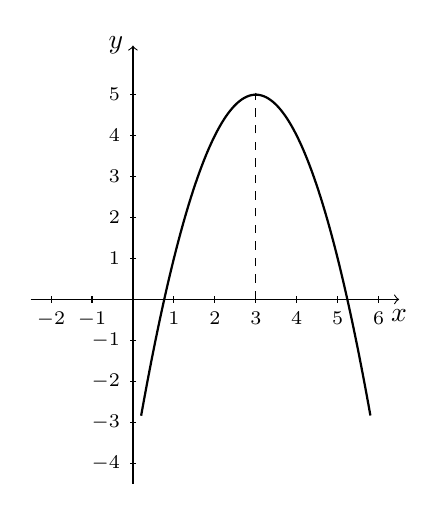
\begin{tikzpicture}[scale=0.52]
    \draw[->] (-2.5,0) -- (6.5,0) node[below] {$x$};
    \draw[->] (0,-4.5) -- (0,6.2) node[left] {$y$};
    \foreach \x in {-2,-1,1,2,3,4,5,6}
      \draw (\x,0.08)--(\x,-0.08) node[below] {\scriptsize $\x$};
    \foreach \y in {-4,-3,-2,-1,1,2,3,4,5}
      \draw (0.08,\y)--(-0.08,\y) node[left] {\scriptsize $\y$};
    \draw[smooth, samples=200, domain=0.2:5.8, thick] plot (\x, {-(\x-3)*(\x-3)+5});
    \draw[dashed] (3,0) -- (3,5);
    \fill (3,5) circle (1.2pt);
\end{tikzpicture}
